% questions.tex —— 2020 年·全国Ⅰ卷·文科 · 题目内容片段（无答案）
% 由 tools/generate_projects.py 依来源总账自 2020/2020_数学真题_文_试题.md 生成，勿手改（改源 MD 后重跑）


\begin{gknotice}
\textbf{ 卷种提示}

本卷为\textbf{文理分科时代的旧结构}，且含\textbf{现已取消的选做题}（第 22/23 题）与\textbf{已删除的程序框图}考点（第 9 题）。

与同年理科卷有 \textbf{8 题重合}（第 3、5、7、12、13、21、22、23 题），其余题目难度普遍低于理科卷。

学生若为\textbf{物化生方向}，优先使用理科卷；本卷适合作为\textbf{基础巩固}或按知识点抽题。
\end{gknotice}

\par\medskip

\gkpart{一、选择题}

\begin{gktip}
本题共 12 小题，每小题 5 分，共 60 分。
\end{gktip}

\begin{question}
\gkti{1}已知集合 $A=\left\{x\mid x^{2}-3x-4<0\right\}$，$B=\{-4,1,3,5\}$，则 $A\cap B=$（　　）

\begin{gkopts}(4)
\task A．$\{-4,1\}$
\task B．$\{1,5\}$
\task C．$\{3,5\}$
\task D．$\{1,3\}$
\end{gkopts}

\end{question}
\begin{question}
\gkti{2}若 $z=1+2\mathrm i+\mathrm i^{3}$，则 $|z|=$（　　）

\begin{gkopts}(4)
\task A．$0$
\task B．$1$
\task C．$\sqrt2$
\task D．$2$
\end{gkopts}

\end{question}
\begin{question}
\gkti{3}埃及胡夫金字塔是古代世界建筑奇迹之一，它的形状可视为一个正四棱锥，以该四棱锥的高为边长的正方形面积等于该四棱锥一个侧面三角形的面积，则其侧面三角形底边上的高与底面正方形的边长的比值为（　　）

\begin{gkopts}(2)
\task A．$\dfrac{\sqrt5-1}4$
\task B．$\dfrac{\sqrt5-1}2$
\task C．$\dfrac{\sqrt5+1}4$
\task D．$\dfrac{\sqrt5+1}2$
\end{gkopts}

\end{question}
\begin{question}
\gkti{4}设 $O$ 为正方形 $ABCD$ 的中心，在 $O$，$A$，$B$，$C$，$D$ 中任取 $3$ 点，则取到的 $3$ 点共线的概率为（　　）

\begin{gkopts}(4)
\task A．$\dfrac15$
\task B．$\dfrac25$
\task C．$\dfrac12$
\task D．$\dfrac45$
\end{gkopts}

\Needspace{0.4\textheight}
\end{question}
\begin{question}
\gkti{5}某校一个课外学习小组为研究某作物种子的发芽率 $y$ 和温度 $x$（单位：$^\circ\mathrm C$）的关系，在 $20$ 个不同的温度条件下进行种子发芽实验，得到下面的散点图：
\nopagebreak[4]
\begin{center}% 2020 全国Ⅰ卷 理5：发芽率-温度散点图（对数饱和形态，数据点按原图形态示意布点）
\begin{tikzpicture}
\begin{axis}[width=8.8cm, height=5cm, font=\small,
  xlabel={温度$/^{\circ}\mathrm{C}$}, ylabel={发芽率},
  xlabel style={at={(1,0)}, anchor=north west},
  ylabel style={at={(0,1)}, anchor=south, rotate=-90},
  xmin=0, xmax=44, ymin=0, ymax=1.08,
  xtick={0,10,20,30,40},
  ytick={0.2,0.4,0.6,0.8,1.0},
  yticklabels={$20\%$,$40\%$,$60\%$,$80\%$,$100\%$},
  axis lines=left, axis line style={-Stealth}]
  \addplot[only marks, mark=square*, mark size=1.3pt] coordinates {
    (10,0.36) (11.5,0.42) (13,0.50) (14.5,0.55) (16,0.58)
    (17.5,0.62) (19,0.64) (20.5,0.68) (22,0.69) (23.5,0.72)
    (25,0.73) (26.5,0.76) (28,0.76) (29.5,0.79) (31,0.80)
    (33,0.82) (35,0.83) (37,0.86) (39,0.86) (40.5,0.88)};
  \addplot[domain=9:41, samples=80, smooth] {0.35*ln(x)-0.45};
\end{axis}
\end{tikzpicture}
\end{center}
\nopagebreak[4]
由此散点图，在 $10\ ^\circ\mathrm C$ 至 $40\ ^\circ\mathrm C$ 之间，下面四个回归方程类型中最适宜作为发芽率 $y$ 和温度 $x$ 的回归方程类型的是（　　）

\begin{gkopts}(2)
\task A．$y=a+bx$
\task B．$y=a+bx^{2}$
\task C．$y=a+b\mathrm e^{x}$
\task D．$y=a+b\ln x$
\end{gkopts}

\end{question}
\begin{question}
\gkti{6}已知圆 $x^{2}+y^{2}-6x=0$，过点 $(1,2)$ 的直线被该圆所截得的弦的长度的最小值为（　　）

\begin{gkopts}(4)
\task A．$1$
\task B．$2$
\task C．$3$
\task D．$4$
\end{gkopts}

\Needspace{0.4\textheight}
\end{question}
\begin{question}
\gkti{7}设函数 $f(x)=\cos\left(\omega x+\dfrac\pi6\right)$ 在 $[-\pi,\pi]$ 的图象大致如下图，则 $f(x)$ 的最小正周期为（　　）
\nopagebreak[4]
\begin{center}% 2020 全国Ⅰ卷 理7：f(x)=cos(ωx+π/6) 的图象（按答案 T=4π/3，即 ω=3/2 精确绘制）
\begin{tikzpicture}
\begin{axis}[width=8.6cm, height=4.6cm, font=\small,
  axis lines=middle, xlabel={$x$}, ylabel={$y$},
  xmin=-3.6, xmax=3.7, ymin=-1.35, ymax=1.45,
  xtick={-3.14159, -1.39626, 3.14159},
  xticklabels={$-\pi$, $-\frac{4\pi}{9}$, $\pi$},
  ytick=\empty,
  every axis x label/.style={at={(current axis.right of origin)}, anchor=west},
  every axis y label/.style={at={(current axis.above origin)}, anchor=south}]
  \addplot[domain=-3.14159:3.14159, samples=200, thick] {cos(deg(1.5*x + pi/6))};
  \node[below left, font=\small] at (axis cs:0,0) {$O$};
\end{axis}
\end{tikzpicture}
\end{center}
\nopagebreak[4]
\begin{gkopts}(4)
\task A．$\dfrac{10\pi}9$
\task B．$\dfrac{7\pi}6$
\task C．$\dfrac{4\pi}3$
\task D．$\dfrac{3\pi}2$
\end{gkopts}

\end{question}
\begin{question}
\gkti{8}设 $a\log_3 4=2$，则 $4^{-a}=$（　　）

\begin{gkopts}(4)
\task A．$\dfrac1{16}$
\task B．$\dfrac19$
\task C．$\dfrac18$
\task D．$\dfrac16$
\end{gkopts}

\Needspace{0.4\textheight}
\end{question}
\begin{question}
\gkti{9}执行下面的程序框图，则输出的 $n=$（　　）
\nopagebreak[4]
\begin{center}% 2020 全国Ⅰ卷 文9：累加程序框图（输出 n=17）
\begin{tikzpicture}[font=\small, >=Stealth, node distance=7mm,
  box/.style={draw, minimum height=1.9em, inner xsep=7pt},
  term/.style={draw, rounded corners=7pt, minimum height=1.9em, inner xsep=9pt},
  io/.style={draw, trapezium, trapezium left angle=70, trapezium right angle=110,
             minimum height=1.9em, inner xsep=2pt},
  dec/.style={draw, diamond, aspect=2.4, inner sep=1.5pt}]
  \node[term] (start) {开始};
  \node[box, below=of start] (init) {$n=1$，$S=0$};
  \coordinate[below=4mm of init] (merge);
  \node[box, below=2mm of merge] (acc) {$S=S+n$};
  \node[dec, below=of acc] (cond) {$S\le100$};
  \node[box, left=12mm of acc, minimum width=5.2em] (inc) {$n=n+2$};
  \node[io, below=of cond] (out) {输出 $n$};
  \node[term, below=of out] (end) {结束};
  \draw[->] (start) -- (init);
  \draw[->] (init) -- (acc);
  \draw[->] (acc) -- (cond);
  \draw[->] (cond) -- node[right]{否} (out);
  \draw[->] (out) -- (end);
  \draw[->] (cond) -| node[below, pos=0.18]{是} (inc);
  \draw[->] (inc) |- (merge);
\end{tikzpicture}
\end{center}
\nopagebreak[4]
\begin{gkopts}(4)
\task A．$17$
\task B．$19$
\task C．$21$
\task D．$23$
\end{gkopts}

\begin{gktip}
\textbf{注}：程序框图（算法初步）在现行新课标中已删除，本题仅作历史资料保留。
\end{gktip}

\end{question}
\begin{question}
\gkti{10}设 $\left\{a_n\right\}$ 是等比数列，且 $a_1+a_2+a_3=1$，$a_2+a_3+a_4=2$，则 $a_6+a_7+a_8=$（　　）

\begin{gkopts}(4)
\task A．$12$
\task B．$24$
\task C．$30$
\task D．$32$
\end{gkopts}

\end{question}
\begin{question}
\gkti{11}设 $F_1$，$F_2$ 是双曲线 $C:x^{2}-\dfrac{y^{2}}3=1$ 的两个焦点，$O$ 为坐标原点，点 $P$ 在 $C$ 上且 $|OP|=2$，则 $\triangle PF_1F_2$ 的面积为（　　）

\begin{gkopts}(4)
\task A．$\dfrac72$
\task B．$3$
\task C．$\dfrac52$
\task D．$2$
\end{gkopts}

\end{question}
\begin{question}
\gkti{12}已知 $A$，$B$，$C$ 为球 $O$ 的球面上的三个点，$\odot O_1$ 为 $\triangle ABC$ 的外接圆。若 $\odot O_1$ 的面积为 $4\pi$，$AB=BC=AC=OO_1$，则球 $O$ 的表面积为（　　）

\begin{gkopts}(4)
\task A．$64\pi$
\task B．$48\pi$
\task C．$36\pi$
\task D．$32\pi$
\end{gkopts}

\par\medskip

\end{question}
\gkpart{二、填空题}

\begin{gktip}
本题共 4 小题，每小题 5 分，共 20 分。
\end{gktip}

\begin{question}
\gkti{13}若 $x$，$y$ 满足约束条件 $\begin{cases}2x+y-2\le0\\ x-y-1\ge0\\ y+1\ge0\end{cases}$，则 $z=x+7y$ 的最大值为 \gkblank{}．

\end{question}
\begin{question}
\gkti{14}设向量 $\boldsymbol a=(1,-1)$，$\boldsymbol b=(m+1,\ 2m-4)$，若 $\boldsymbol a\perp\boldsymbol b$，则 $m=$ \gkblank{}．

\end{question}
\begin{question}
\gkti{15}曲线 $y=\ln x+x+1$ 的一条切线的斜率为 $2$，则该切线的方程为 \gkblank{}．

\end{question}
\begin{question}
\gkti{16}数列 $\left\{a_n\right\}$ 满足 $a_{n+2}+(-1)^{n}a_n=3n-1$，前 $16$ 项和为 $540$，则 $a_1=$ \gkblank{}．

\par\medskip

\end{question}
\gkpart{三、解答题}

\begin{gktip}
共 70 分。第 17～21 题为必考题，第 22、23 题为选考题。
\end{gktip}

\gksubpart{（一）必考题：共 60 分}

\begin{question}
\gkti{17}\textbf{（12 分）} 某厂接受了一项加工业务，加工出来的产品（单位：件）按标准分为 $A$，$B$，$C$，$D$ 四个等级。加工业务约定：对于 $A$ 级品、$B$ 级品、$C$ 级品，厂家每件分别收取加工费 $90$ 元、$50$ 元、$20$ 元；对于 $D$ 级品，厂家每件要赔偿原料损失费 $50$ 元。该厂有甲、乙两个分厂可承接加工业务。甲分厂加工成本费为 $25$ 元/件，乙分厂加工成本费为 $20$ 元/件。厂家为决定由哪个分厂承接加工业务，在两个分厂各试加工了 $100$ 件这种产品，并统计了这些产品的等级，整理如下：

\textbf{甲分厂产品等级的频数分布表}

\begin{center}
\begin{tabular}{ccccc}
\toprule
等级 & $A$ & $B$ & $C$ & $D$ \\
\midrule
频数 & $40$ & $20$ & $20$ & $20$ \\
\bottomrule
\end{tabular}
\end{center}

\textbf{乙分厂产品等级的频数分布表}

\begin{center}
\begin{tabular}{ccccc}
\toprule
等级 & $A$ & $B$ & $C$ & $D$ \\
\midrule
频数 & $28$ & $17$ & $34$ & $21$ \\
\bottomrule
\end{tabular}
\end{center}

  (1) 分别估计甲、乙两分厂加工出来的一件产品为 $A$ 级品的概率；

  (2) 分别求甲、乙两分厂加工出来的 $100$ 件产品的平均利润，以平均利润为依据，厂家应选哪个分厂承接加工业务？

\end{question}
\begin{question}
\gkti{18}\textbf{（12 分）} $\triangle ABC$ 的内角 $A$，$B$，$C$ 的对边分别为 $a$，$b$，$c$。已知 $B=150^\circ$。

  (1) 若 $a=\sqrt3c$，$b=2\sqrt7$，求 $\triangle ABC$ 的面积；

  (2) 若 $\sin A+\sqrt3\sin C=\dfrac{\sqrt2}2$，求 $C$。

\Needspace{0.4\textheight}
\end{question}
\begin{question}
\gkti{19}\textbf{（12 分）} 如图，$D$ 为圆锥的顶点，$O$ 是圆锥底面的圆心，$\triangle ABC$ 是底面的内接正三角形，$P$ 为 $DO$ 上一点，$\angle APC=90^\circ$。
\nopagebreak[4]
\begin{center}% 2020 全国Ⅰ卷 文19：圆锥（顶点 D，圆心 O，△ABC 内接正三角形，P 在 DO 上，∠APC=90°）
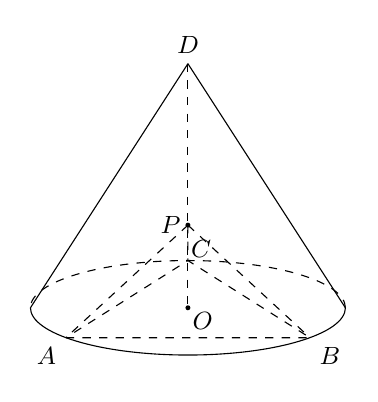
\begin{tikzpicture}[scale=1.0, font=\small]
  \coordinate (D) at (0,3.1);
  \coordinate (O) at (0,0);
  \coordinate (A) at (-1.55,-0.38);
  \coordinate (B) at (1.55,-0.38);
  \coordinate (C) at (0,0.6);
  \coordinate (P) at (0,1.05);
  \draw (-2,0) arc (180:360:2 and 0.6);
  \draw[dashed] (2,0) arc (0:180:2 and 0.6);
  \draw (D) -- (-2,0);
  \draw (D) -- (2,0);
  \draw[dashed] (D) -- (O);
  \draw[dashed] (A) -- (B) -- (C) -- cycle;
  \draw[dashed] (P) -- (A)  (P) -- (B)  (P) -- (C);
  \fill (O) circle (0.9pt);  \fill (P) circle (0.9pt);
  \node[above] at (D) {$D$};
  \node[below left] at (A) {$A$};
  \node[below right] at (B) {$B$};
  \node[above right, inner sep=1pt] at (C) {$C$};
  \node[below right, inner sep=1.5pt] at (O) {$O$};
  \node[left, inner sep=2.5pt] at (P) {$P$};
\end{tikzpicture}
\end{center}
\nopagebreak[4]
  (1) 证明：平面 $PAB\perp$ 平面 $PAC$；

  (2) 设 $DO=\sqrt2$，圆锥的侧面积为 $\sqrt3\pi$，求三棱锥 $P\text{-}ABC$ 的体积。

\end{question}
\begin{question}
\gkti{20}\textbf{（12 分）} 已知函数 $f(x)=\mathrm e^{x}-a(x+2)$。

  (1) 当 $a=1$ 时，讨论 $f(x)$ 的单调性；

  (2) 若 $f(x)$ 有两个零点，求 $a$ 的取值范围。

\end{question}
\begin{question}
\gkti{21}\textbf{（12 分）} 已知 $A$，$B$ 分别为椭圆 $E:\dfrac{x^{2}}{a^{2}}+y^{2}=1\ (a>1)$ 的左、右顶点，$G$ 为 $E$ 的上顶点，$\overrightarrow{AG}\cdot\overrightarrow{GB}=8$，$P$ 为直线 $x=6$ 上的动点，$PA$ 与 $E$ 的另一交点为 $C$，$PB$ 与 $E$ 的另一交点为 $D$。

  (1) 求 $E$ 的方程；

  (2) 证明：直线 $CD$ 过定点。

\par\medskip

\end{question}
\gksubpart{（二）选考题：共 10 分，第 22、23 题任选一题作答}

\begin{gktip}
\textbf{ 现行考纲已取消选做题}，以下两题仅作历史资料保留，不建议练习。
\end{gktip}

\begin{question}
\gkti{22}\textbf{（10 分）〔选修 4-4：坐标系与参数方程〕} （\textbf{已取消}）

在直角坐标系 $xOy$ 中，曲线 $C_1$ 的参数方程为 $\begin{cases}x=\cos^{k}t\\ y=\sin^{k}t\end{cases}$（$t$ 为参数）。以坐标原点为极点，$x$ 轴正半轴为极轴建立极坐标系，曲线 $C_2$ 的极坐标方程为 $4\rho\cos\theta-16\rho\sin\theta+3=0$。

  (1) 当 $k=1$ 时，$C_1$ 是什么曲线？

  (2) 当 $k=4$ 时，求 $C_1$ 与 $C_2$ 的公共点的直角坐标。

\end{question}
\begin{question}
\gkti{23}\textbf{（10 分）〔选修 4-5：不等式选讲〕} （\textbf{已取消}）

已知函数 $f(x)=|3x+1|-2|x-1|$。

  (1) 画出 $y=f(x)$ 的图象；

  (2) 求不等式 $f(x)>f(x+1)$ 的解集。

\par\medskip


\end{question}